\documentclass[12pt, a4paper, twoside]{article}

%% Preamble
\usepackage{umatfgenglish}
\usepackage{blindtext}
\usepackage{amssymb}
\usepackage{amsmath}
\usepackage{graphicx}
\graphicspath{ {./images/} }

\begin{document}

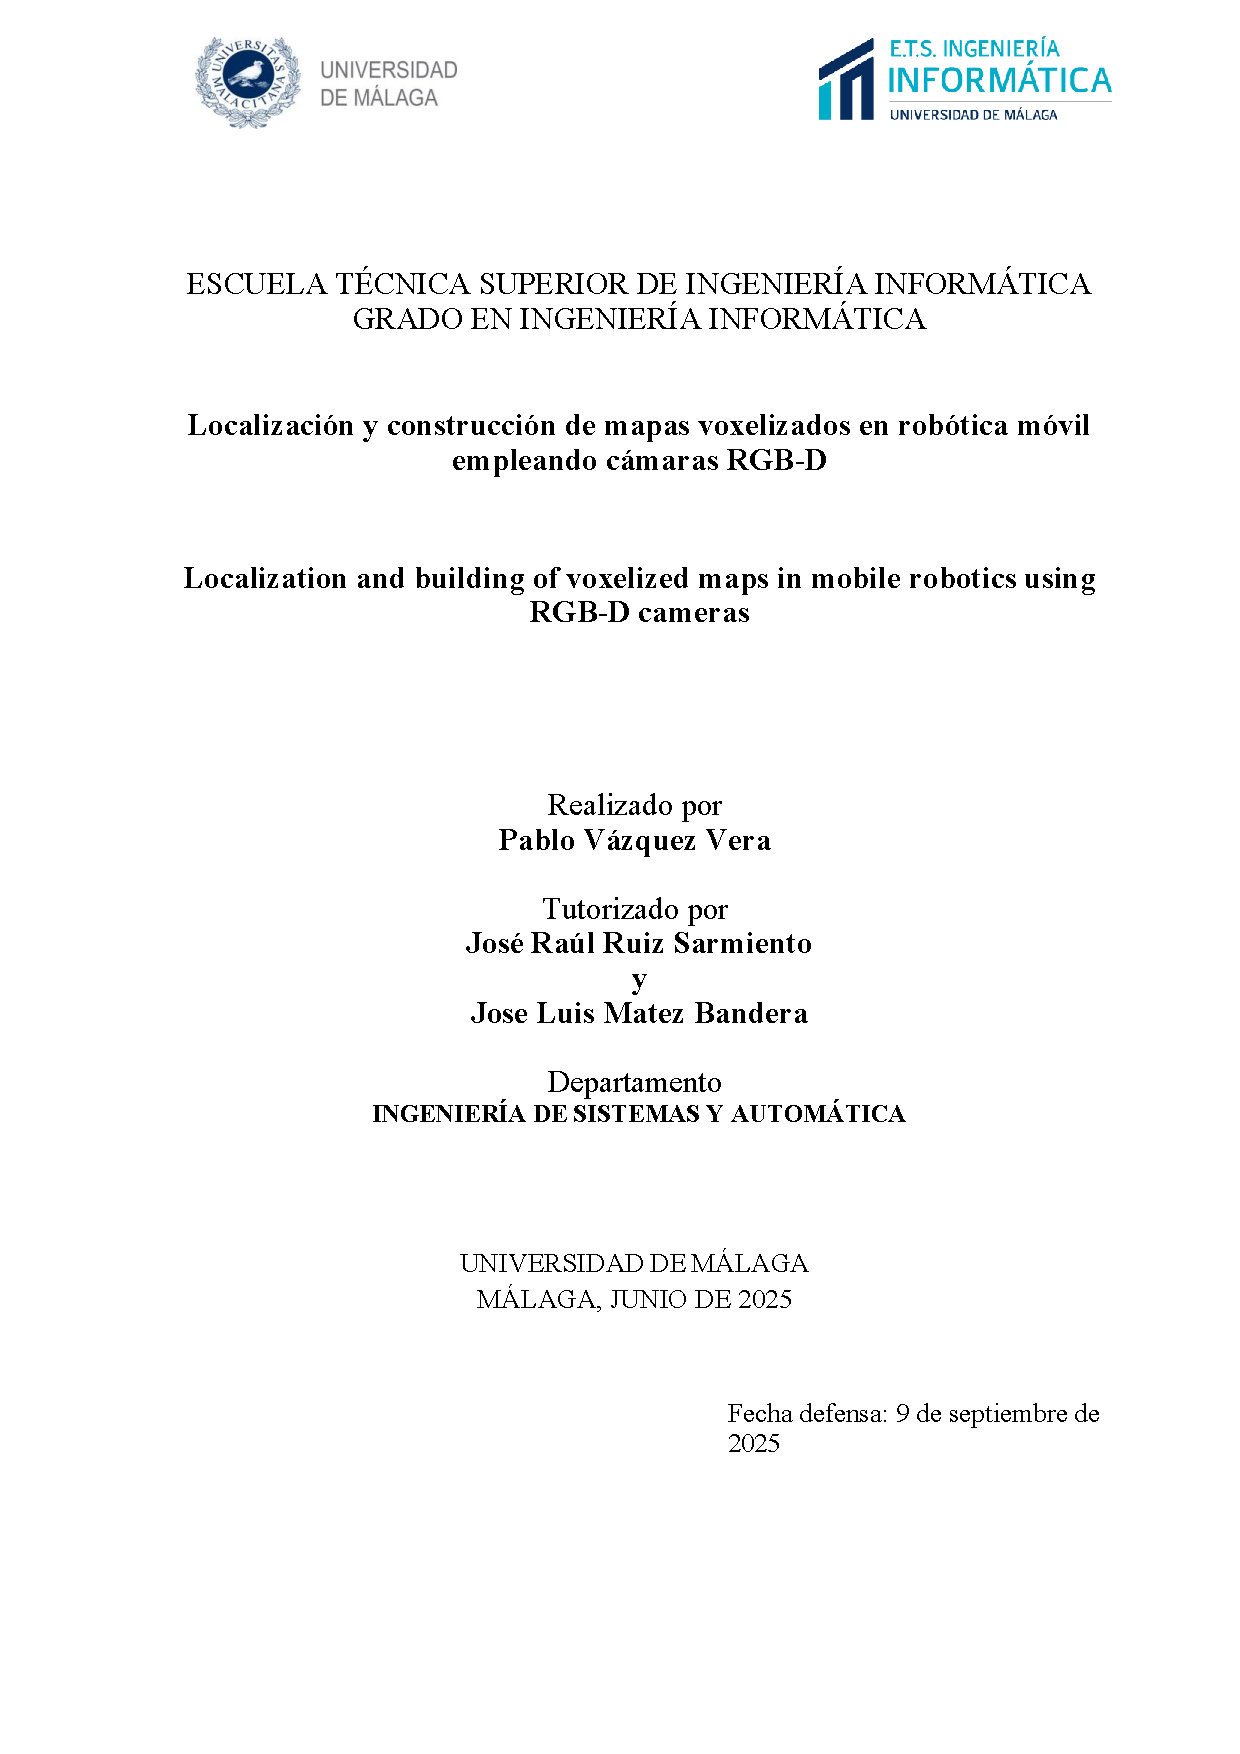
\includepdf[noautoscale=true, width=\paperwidth]{title.pdf}

\newpage

%% Abstract
\begin{abstract}
  La robótica es una disciplina que ha crecido en los últimos años, y su aplicación en la industria ha demostrado ser muy 
  beneficiosa en gran cantidad de materias. Desde la automatización de tareas repetitivas hasta la mejora de la precisión en 
  procesos de manufactura, los robots han revolucionado la forma en que realizamos todo tipo de tareas, algunas inconcebibles 
  tan solo unos años atrás. \newline
  En el campo de la robótica existen diversas ramas, cada una con su propio enfoque y aplicación. Una de estas ramas es la robótica 
  móvil, que se centra en el diseño y desarrollo de robots capaces de moverse de manera autónoma en entornos dinámicos. 
  La robótica móvil ha encontrado aplicaciones en una amplia variedad de campos, desde la exploración espacial hasta la logística 
  y el transporte. \newline
  En este contexto, el presente documento tiene como objetivo investigar y analizar la viabilidad de un proyecto de robótica móvil, 
  centrado en la creación de un robot capaz de localizarse de manera autónoma en un entorno desconocido a la vez que genera un mapa 
  voxelizado de este, recibiendo como única fuente de datos nubes de puntos capturadas del entorno. Exploraremos los desafíos 
  técnicos y las oportunidades que presenta este proyecto, así como su potencial impacto en la industria 
  y la sociedad en general. \newline

  \bfseries{\large{Palabras clave:}}
  Robótica móvil, Navegación autónoma, Mapas voxelizados, Nubes de puntos, Exploración de entornos desconocidos.
\end{abstract}

\tableofcontents

%% Sections
\section{Introducción}

\subsection{Motivación}
La robótica es una disciplina que ha ensanchado sus fronteras en los últimos años, y su aplicación en la industria ha demostrado ser 
increíblemente beneficiosa en gran cantidad de materias, atrayendo la atención tanto de investigadores y profesionales de todo el 
mundo como de empresas e inversores interesados en su desarrollo y aplicación. \newline
Una de las ramas más prometedoras de la robótica es la robótica móvil, que se centra en el diseño y desarrollo de robots capaces 
de moverse de manera autónoma en entornos dinámicos. Esta rama es una de las más complejas y a la vez fascinantes, ya que implica 
la integración de diversas disciplinas como la inteligencia artificial, la visión por computadora y el control de sistemas que 
deben trabajar en perfecta sintonía para lograr que el robot sea capaz de navegar y operar de manera eficiente en entornos que 
pueden ser impredecibles y cambiantes. \newline
La tarea que nos ocupa en este documento es la creación de un robot capaz de localizarse de manera autónoma en un entorno 
desconocido a la vez que genera un mapa voxelizado de este. Para llevar a cabo esta tarea, el robot recibirá como única fuente 
de datos nubes de puntos capturadas del entorno. \newline
Este proyecto plantea una serie de desafíos ligados a la naturaleza de los datos que se utilizan, ya que las nubes de puntos son 
representaciones tridimensionales del entorno que pueden ser:  
\begin{itemize}
  \item  \textbf{Computacionalmente costosas}: 
    Las nubes de puntos pueden contener millones de puntos, lo que requiere un procesamiento intensivo para extraer información útil.
  \item  \textbf{Ruidosas}:
    Las nubes de puntos pueden contener ruido debido a errores en la captura de datos intrínsecos a la naturaleza de los sensores.
  \item  \textbf{Incompletas}:
    Las nubes de puntos pueden no representar completamente el entorno debido a limitaciones en la cobertura del sensor o a 
    obstrucciones físicas en el entorno.
\end{itemize}
\begin{figure}[h]
  \centering
    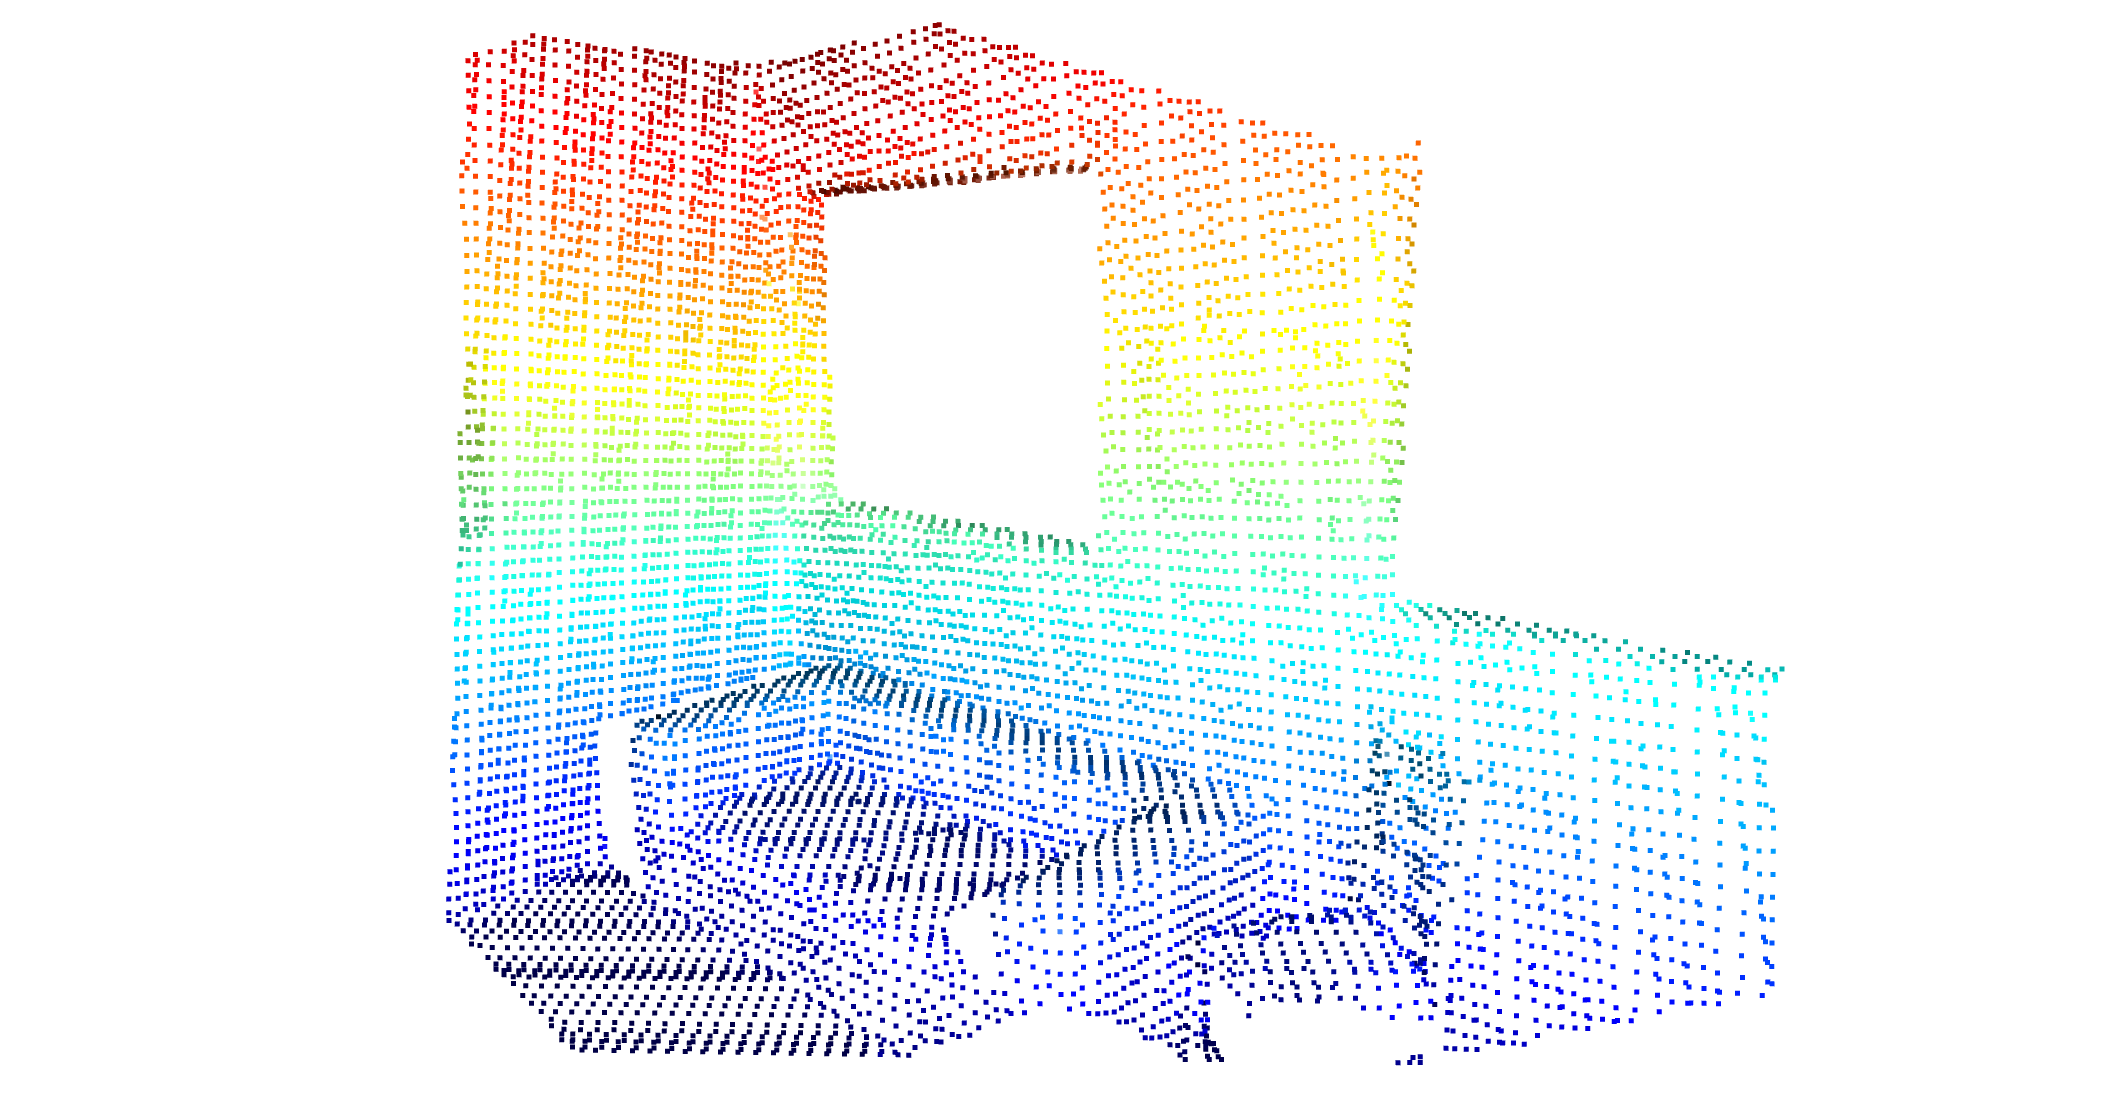
\includegraphics[width=0.5\textwidth]{Point_cloud_example.png}
  \caption{Imagen de una nube de puntos.}
\end{figure}
Esto nos llevará a explorar diversas técnicas de procesamiento de datos y algoritmos de localización y mapeo, así como a 
considerar las limitaciones y oportunidades que presenta el uso de nubes de puntos y los mapas voxelizados en la 
robótica móvil. \newline
Entre las herramientas y técnicas de interés más destacadas relacionadas con la casuística que tratamos encontraremos 
el uso de ICP (Iterative Closest Point) para la alineación de nubes de puntos y, por consiguiente, la obtención de la pose relativa, 
Bonxai para la generación, manipulación y almacenamiento de mapas voxelizados gestionados de manera eficiente y aprovecharemos 
la amplia gama de herramientas y bibliotecas proporcionadas por ROS en su segunda versión, ROS2, para la implementación de los 
algoritmos de localización y mapeo, así como la potencia y versatilidad de lenguajes de programación como Python y C++. \newline

\begin{figure}[h]
  \centering
    
\includegraphics[width=0.5\textwidth]{ROS2_logo.png}
  \caption{Logo de la plataforma ROS2 [1].}
\end{figure}

\subsection{Objetivos}

El objetivo principal de este proyecto es desarrollar un robot capaz de localizarse de manera autónoma en un entorno desconocido y 
generar un mapa voxelizado de este entorno utilizando nubes de puntos como única fuente de datos. Para lograr este objetivo, se ha 
de llevar a cabo una serie de tareas específicas:
\begin{itemize}
  \item \textbf{Diseño de un flujo de trabajo.} Para desarrollar este flujo de trabajo es necesario diseñar:
   \begin{itemize}
    \item \textbf{Sincronización de mensajes:} Se debe establecer un mecanismo de sincronización que permita 
      recibir y procesar las nubes de puntos de manera eficiente, asegurando que los datos estén disponibles en el momento 
      adecuado para su procesamiento. Además, se debe considerar cómo se gestionará la comunicación entre los diferentes 
      componentes del sistema, incluyendo la adquisición de datos, el procesamiento, localización y la generación del mapa.
    \item \textbf{Preprocesamiento de los datos:} Se debe realizar un preprocesamiento de las nubes de puntos 
      para eliminar ruido y mejorar la calidad de los datos. Esto puede incluir técnicas como filtrado, segmentación y 
      reducción de ruido, así como la normalización de los datos para facilitar su procesamiento posterior.
    \item \textbf{Cálculo de la pose:} Se debe implementar un algoritmo que permita calcular la pose del robot en el entorno 
      a partir de las nubes de puntos recibidas. Esto puede incluir técnicas como ICP (Iterative Closest Point) para 
      alinear las nubes de puntos y estimar la pose relativa del robot.
    \item \textbf{Construcción del mapa voxelizado:} Se debe utilizar alguna herramienta para la generación y manipulación 
      de mapas voxelizados, como Bonxai, para crear un mapa del entorno a partir de las nubes de puntos procesadas. 
      Esto puede incluir la creación de una estructura de datos eficiente para almacenar el mapa y la implementación de 
      algoritmos para actualizar el mapa a medida que se reciben nuevas nubes de puntos.
    \end{itemize}
  \item \textbf{Procedimiento de validación:} Es necesario estudiar y definir un procedimiento que permita evaluar de manera 
    objetiva la precisión y eficiencia del sistema de localización y mapeo desarrollado. Este procedimiento debe incluir:
    \begin{itemize}
    \item \textbf{Definición de métricas sobre la calidad de la localización:} Se deben definir métricas que permitan evaluar 
      la precisión de la localización del robot en el entorno, considerando factores como la desviación respecto a la posición 
      real y la estabilidad de la localización a lo largo del tiempo.
    \item \textbf{Definición de métricas sobre la calidad del mapa:} Se deben definir métricas que permitan evaluar la calidad 
      del mapa generado por el robot, considerando factores como la capacidad de representar adecuadamente el entorno.
    \item \textbf{Comparativa entre enfoques:} Se debe realizar una comparativa entre los diferentes enfoques desarrollados 
      en el proyecto, evaluando su rendimiento y eficiencia en función de las métricas definidas anteriormente.
    \end{itemize}
\end{itemize}

\subsection{Estructura del documento}

La estructura del documento se organiza en 6 capítulos principales, cada uno de los cuales aborda un aspecto clave del proyecto:
\begin{itemize}
  \item \textbf{Capítulo 1: Introducción.} En este capítulo se presenta el contexto del proyecto, qué motiva el 
    desarrollo y la investigación llevada a cabo, así como se definen una serie de objetivos que se pretenden alcanzar.
  \item \textbf{Capítulo 2: Bases.} En este capítulo se proporciona una visión general de las bases teóricas y 
    técnicas que sustentan el proyecto, incluyendo conceptos clave como la localización, el mapeo y las nubes de puntos.
  \item \textbf{Capítulo 3: Tecnologías usadas.} En este capítulo se describen las tecnologías y herramientas utilizadas 
    en el proyecto, incluyendo ROS2 y Bonxai, entre otros. Además, se presentan las ventajas y desventajas de cada una de ellas, 
    así como su aplicabilidad en el contexto del proyecto.
  \item \textbf{Capítulo 4: Localización y mapeo.} Este capítulo se centra en los algoritmos y técnicas utilizados para 
    la localización y el mapeo del robot en un entorno desconocido, incluyendo la alineación de nubes de puntos y la generación 
    de mapas voxelizados.
  \item \textbf{Capítulo 5: Validación de resultados.} En este capítulo se presentan los resultados obtenidos en el proyecto, 
    incluyendo la evaluación de la precisión y eficiencia del sistema de localización y mapeo, así como una comparativa entre 
    los enfoques desarrollados.
  \item \textbf{Capítulo 6: Conclusiones.} En este capítulo se presentan las conclusiones del proyecto, incluyendo una reflexión 
    sobre los logros alcanzados, las lecciones aprendidas y las posibles direcciones futuras de investigación y desarrollo en el 
    campo de la robótica móvil.
\end{itemize}

\newpage

\section{Bases}

\subsection{Mapas voxelizados}

\subsubsection{Introducción a los mapas voxelizados}
La idea de los mapas voxelizados surgió como una extensión natural de los conceptos utilizados en la representación 
de imágenes digitales en dos dimensiones, aplicados al espacio tridimensional. Mientras que una imagen está compuesta 
por píxeles (elementos de imagen), un volumen tridimensional puede representarse mediante vóxeles (volumetric pixels), 
es decir, pequeñas celdas cúbicas que subdividen el espacio en una cuadrícula regular. \newline
Este enfoque se originó en el ámbito de la visualización médica y científica durante las décadas de 1970 y 1980, 
cuando surgió la necesidad de modelar órganos y estructuras internas del cuerpo humano a partir de escáneres como la 
tomografía computarizada (CT) y la resonancia magnética (MRI). Posteriormente, el concepto fue adoptado por otras 
disciplinas como la computación gráfica, la simulación física y, más recientemente, la robótica, donde los mapas 
voxelizados se utilizan para representar entornos 3D en tareas de navegación, percepción y planificación de movimiento.
\begin{figure}[h]
  \centering
    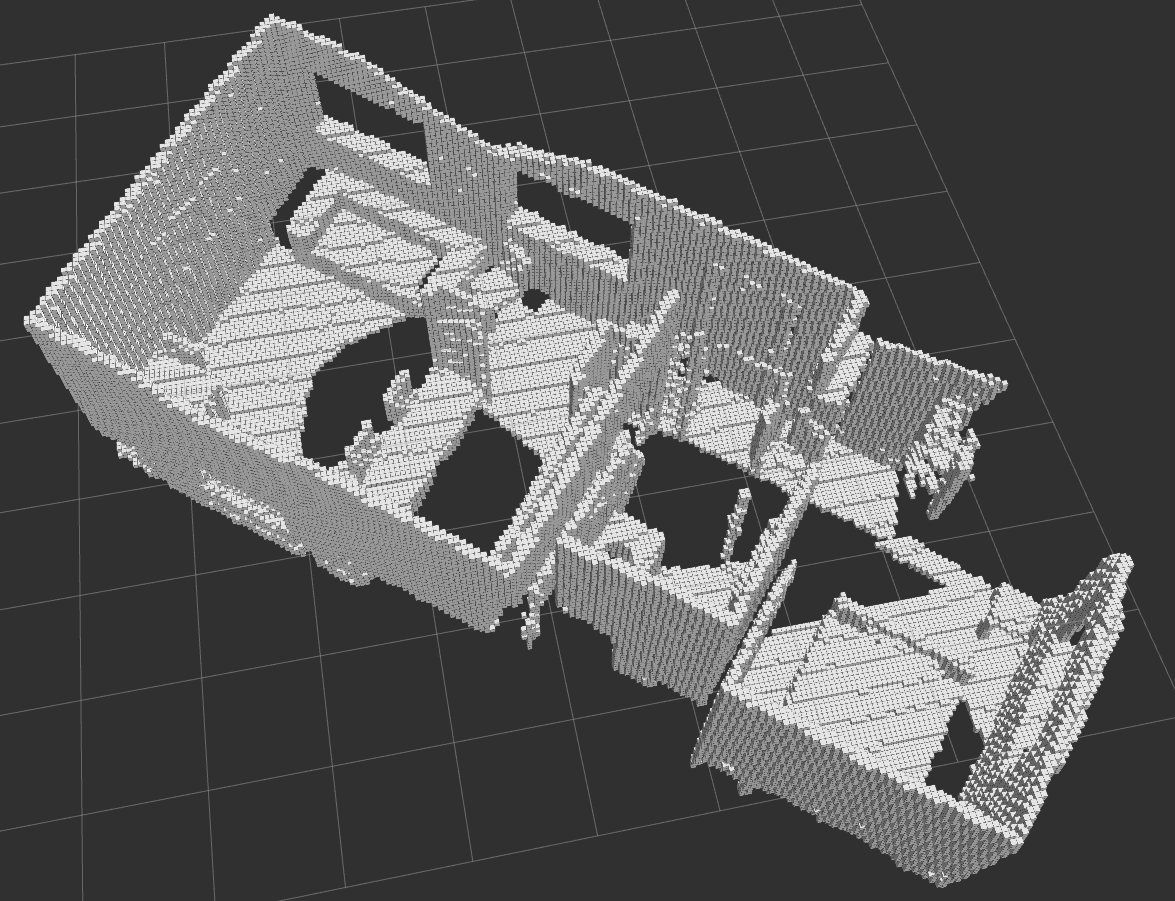
\includegraphics[width=0.5\textwidth]{Voxel_map_example.png}
  \caption{Imagen de un mapa voxelizado.}
\end{figure} 
\newline
Los mapas voxelizados representan una evolución significativa en la forma en que se modelan y procesan entornos 
tridimensionales y su desarrollo está vinculado al crecimiento de la capacidad computacional y la necesidad de 
representar espacios complejos de manera eficiente, especialmente en contextos donde se requiere análisis espacial preciso, 
como en navegación autónoma o reconstrucción 3D.

\subsubsection{Características de los mapas voxelizados}

Un mapa voxelizado divide un espacio tridimensional en una cuadrícula regular de celdas cúbicas, denominadas voxels 
(volumetric pixels). Cada voxel puede contener información binaria (ocupado/libre), probabilística (por ejemplo, con modelos 
bayesianos como los octomapas), o datos más complejos como intensidad, color, o etiquetas semánticas. Entre sus características 
principales se destacan:

\begin{itemize}
  \item \textbf{Representación volumétrica discreta:} Los mapas voxelizados dividen el espacio tridimensional en una rejilla cúbica 
  regular compuesta por pequeñas celdas llamadas voxeles. Cada voxel representa una porción del espacio con una resolución 
  determinada, lo que permite una representación explícita del volumen y no solo de la superficie.
  \item \textbf{Resolución configurable:} La resolución del mapa puede ajustarse modificando el tamaño de los voxeles. Una 
  resolución más alta (voxeles más pequeños) proporciona mayor detalle, pero aumenta el consumo de memoria y el coste 
  computacional. Por el contrario, resoluciones más bajas reducen la precisión, pero permiten una operación más eficiente.
  \item \textbf{Estructura espacial regular:} La organización de los datos en una cuadrícula facilita la implementación de 
  algoritmos paralelos y el acceso constante a la información espacial, lo que es útil en cálculos de visibilidad, planificación 
  de trayectorias y simulaciones físicas.
  \item \textbf{Facilidad para representar ocupación:} Cada voxel puede almacenar un valor que indique si el espacio está ocupado, 
  libre o desconocido. Esta propiedad es fundamental para la planificación y la detección de colisiones en robótica y simulación.
  \item \textbf{Extensibilidad de la información por voxel:} Los voxeles pueden contener no solo información binaria (ocupado/libre), 
  sino también:
  \begin{itemize}
    \item \textbf{Probabilidades:} Representando la probabilidad de ocupación de un voxel, lo que permite manejar incertidumbres 
    en la percepción.
    \item \textbf{Intensidad o color:} Almacenar información adicional como la intensidad de la señal o el color asociado a cada voxel, 
    lo que es útil en aplicaciones de visión por computadora y reconstrucción 3D.
    \item \textbf{Etiquetas semánticas:} Asignar etiquetas a los voxeles para identificar objetos o características del entorno, 
    lo que es especialmente útil en aplicaciones de robótica móvil y percepción semántica.
    \item \textbf{Normales de superficie:} Almacenar información sobre la orientación de las superficies dentro de los voxeles, 
    lo que es útil para la reconstrucción de superficies y la simulación física.
    \end{itemize}
    \item \textbf{Compatibilidad con estructuras jerárquicas:} Para mejorar la eficiencia en almacenamiento y consultas, los mapas 
    voxelizados pueden implementarse con estructuras jerárquicas como los octrees, que dividen el espacio de forma adaptativa según 
    la densidad de información.
    \item  \textbf{Eficiencia en consultas espaciales:} Gracias a su estructura regular (o jerárquica en el caso de octrees), 
    los mapas voxelizados permiten realizar operaciones como:
    \begin{itemize}
    \item \textbf{Búsqueda de vecinos:} Encontrar voxeles adyacentes de manera eficiente.
    \item \textbf{Intersección de rayos:} Determinar si un rayo intersecta con algún voxel, lo que es útil en 
    simulaciones de iluminación y trazado de rayos.
    \item \textbf{Colisiones:} Detectar colisiones entre objetos y el entorno representado por el mapa voxelizado, 
    lo que es esencial en robótica y simulación física.
    \end{itemize}
    \item \textbf{Idoneidad para entornos dinámicos:} La representación voxelizada puede actualizarse de forma local cuando se detectan 
    cambios en el entorno, lo que permite mantener mapas actualizados en tiempo real, aspecto esencial para aplicaciones robóticas y 
    vehículos autónomos.
  \end{itemize}

\subsubsection{Aplicaciones de los mapas voxelizados}
El uso de los mapas voxelizados se ha ampliado a diversos campos con el paso del tiempo gracias a las mejoras en computación, 
tecnologías de captura de datos e inversiones en investigación y desarrollo del área. Algunas de las aplicaciones más 
destacadas incluyen:

\begin{itemize}
  \item \textbf{Robótica móvil y navegación autónoma:} Los mapas voxelizados se utilizan para representar el entorno tridimensional 
  de un robot o vehículo autónomo. Se emplean para la planificación de trayectorias, detección de obstáculos y navegación segura.
  \begin{itemize}
    \item \textbf{Ventajas:} Permiten representar obstáculos a distintas alturas, útil en entornos no planos. Se integran bien con 
    sensores como LIDAR o cámaras RGB-D. Facilitan el ray tracing para simulaciones de sensores y planificación.
    \item \textbf{Inconvenientes:} Alta demanda de memoria y procesamiento, especialmente en espacios grandes. Requieren mecanismos 
    eficientes de actualización en entornos dinámicos.
  \end{itemize}
  \item \textbf{Reconstrucción 3D de escenas:} Los mapas voxelizados permiten reconstruir entornos tridimensionales desde datos de 
  sensores (escáneres láser, cámaras estereoscópicas, etc.).
  \begin{itemize}
    \item \textbf{Ventajas:} Buen manejo de ruido y fusión de múltiples vistas. Permiten interpolar datos faltantes o parciales 
    de forma robusta.
    \item \textbf{Inconvenientes:} La densidad del modelo puede hacer que sea difícil de almacenar o transmitir. Generalmente 
    se requiere un posprocesamiento para renderizado o análisis.
  \end{itemize}
  \item \textbf{Medicina e imagen biomédica:} Se usan para modelar órganos y tejidos en 3D, a partir de escaneos como tomografía 
  (CT) o resonancia magnética (MRI), permitiendo diagnósticos y planificación quirúrgica.
  \begin{itemize}
    \item \textbf{Ventajas:} Representan estructuras internas de forma precisa y continua. Permiten segmentación automática 
    y simulaciones médicas.
    \item \textbf{Inconvenientes:} Altos requisitos computacionales para procesar volúmenes detallados. Requieren software 
    especializado para su interpretación.
  \end{itemize}
  \item \textbf{Simulación física y entornos virtuales:} Se utilizan en motores de física y simulación para modelar el 
  comportamiento de materiales, fluidos o entornos destructibles.
  \begin{itemize}
    \item \textbf{Ventajas:} Representación volumétrica adecuada para materiales no rígidos o granularidad. Permiten simulaciones 
    dinámicas y realistas de colisiones o fluidos.
    \item \textbf{Inconvenientes:} Simulaciones físicas con vóxeles pueden ser computacionalmente más intensas que con mallas.
  \end{itemize}
  \item \textbf{Videojuegos y gráficos por computadora:} Se usan para construir mundos destructibles o interactivos, como en 
  juegos con estética voxel (por ejemplo, Minecraft).
  \begin{itemize}
    \item \textbf{Ventajas:} Simplicidad para modelar entornos que cambian o se destruyen. Representación directa en memoria 
    de entornos interactivos.
    \item \textbf{Inconvenientes:} Apariencia visual menos realista comparada con modelos basados en polígonos. No adecuados 
    para gráficos de alta fidelidad sin posprocesado.
  \end{itemize}
  \item \textbf{Exploración subterránea y minería:} Los mapas voxelizados se utilizan para representar túneles, cavidades o 
  cuerpos geológicos, permitiendo el análisis y la planificación de rutas de extracción.
  \begin{itemize}
    \item \textbf{Ventajas:} Manejan entornos 3D complejos con estructuras irregulares. Permiten planificación segura en 
    zonas de difícil acceso.
    \item \textbf{Inconvenientes:} Requiere integrar datos de múltiples fuentes con resolución variable. Visualización y 
    análisis pueden ser más complejos que con mapas 2D.
  \end{itemize}
\end{itemize}

\section{Tecnologías usadas}
En esta sección nos centraremos en introducir las tecnologías usadas para el proceso completo de desarrollo del proyecto. 
Hablaremos de los lenguajes de programación utilizados, las plataformas de desarrollo, librerias externas y frameworks usados
a lo largo del proyecto.

\subsection{Lenguajes}
En el desarrollo del proyecto se han utilizado varios lenguajes para abordar diferentes aspectos del sistema.
Entre ellos encontramos:

\begin{itemize}
  \item 
  \begin{minipage}[l]{0.7\textwidth}
    \textbf{Python:} 
      Python es un lenguaje de programación interpretado, de alto nivel y con una sintaxis clara y legible. 
      Fue diseñado para ser fácil de aprender y usar, lo que lo hace ideal tanto para principiantes como para desarrolladores 
      avanzados. Es multiparadigma (soporta programación orientada a objetos, funcional e imperativa) y tiene una gran cantidad 
      de bibliotecas disponibles. La integración de Python en ROS2 permite el desarrollo rápido de prototipos y la implementación
      de algoritmos complejos de procesamiento de datos, control y comunicación entre nodos. Python es el lenguaje principal
      de este proyecto, usado para la implementación de nodos de ROS2, controlando el flujo de datos, la lógica para el cálculo 
      de la pose, métricas de validación y manipulación de nubes de puntos.
  \end{minipage}
  \hspace{1em}
  \begin{minipage}[r]{0.28\textwidth}
    
\includegraphics[width=\linewidth]{Python_logo.png}
  \end{minipage}
  \item \textbf{C++:} C++ es un lenguaje de programación compilado, de propósito general, conocido por su alto rendimiento, 
  control sobre el hardware y capacidades de programación orientada a objetos. Es ampliamente utilizado en sistemas embebidos, 
  videojuegos, y especialmente en aplicaciones donde el rendimiento y la eficiencia son críticos. La integración de C++
  en ROS2 permite el desarrollo de nodos de alto rendimiento, especialmente aquellos que requieren procesamiento intensivo
  de datos o interacción directa con hardware. En este proyecto, C++ se utiliza para nodos de almacenamiento y gestión del
  mapa voxelizado e interacción con la librería Bonxai, que proporciona una interfaz eficiente para la manipulación de mapas
  voxelizados.
  \item \textbf{XML:} XML (eXtensible Markup Language) es un lenguaje de marcado diseñado para almacenar y 
  transportar datos de forma estructurada y legible tanto para humanos como para máquinas. En ROS2, XML se utiliza principalmente 
  en la configuración y descripción de componentes del sistema robótico debido al sistema de descripciones de robots URDF y 
  XACRO, legibilidad, interoperabilidad y amplia adopción en la industria. En este proyecto, XML se utiliza para
  definir la configuración de los nodos de ROS2, incluyendo parámetros, tópicos y dependencias entre servicios.
  \item \textbf{YAML:} YAML (Yet Another Markup Language, o más correctamente YAML Ain't Markup Language) es un formato de 
  serialización de datos basado en texto, muy usado para representar información de forma estructurada y legible por humanos.
  Sus principales usos son como formato de configuración y para el intercambio de datos entre aplicaciones. En ROS2, YAML se 
  utiliza para definir parámetros de nodos, configuraciones de lanzamiento y otros aspectos del sistema robótico. En este proyecto, 
  YAML se utiliza para almacenar configuraciones de nodos, parámetros de algoritmos y otros datos estructurados necesarios para 
  la ejecución del sistema.
  \item \textbf{CMAKE:} CMake es un lenguaje de configuración y scripting especializado para la construcción de software.
  Se usa como herramienta de automatización de compilación que utiliza archivos llamados CMakeLists.txt para describir 
  cómo debe compilarse y enlazarse un proyecto de software. CMake es usado en ROS2 debido a que es la herramienta 
  estándar para la construcción de paquetes y nodos, facilitando la gestión de dependencias, la configuración del entorno
  de compilación y la generación de archivos de configuración necesarios para la ejecución de los nodos desarrollados en C++.
  \item \textbf{LaTeX:} LaTeX es un sistema de composición de documentos basado en el lenguaje de tipografía TeX. Está 
  diseñado para la creación de documentos de alta calidad tipográfica, especialmente aquellos que incluyen fórmulas matemáticas 
  complejas, referencias cruzadas, bibliografías y estructuras organizadas como capítulos, secciones y tablas.
\end{itemize}

\subsection{Entorno, software y herramientas de desarrollo}
  En el desarrollo del proyecto se han utilizado varias herramientas y entornos para facilitar la implementación, el desarrollo
  y la prueba del código. Entre ellos encontramos:
  \begin{itemize}
    \item
      \textbf{ROS2 (Humble Hawksbill):} ROS 2 (Robot Operating System 2) es un marco de desarrollo y un conjunto de herramientas 
      diseñadas para facilitar la creación de sistemas robóticos complejos, modulares y distribuidos. Aunque su nombre sugiere que es 
      un sistema operativo, en realidad ROS 2 no es un sistema operativo tradicional, sino una capa de software que proporciona 
      abstracciones y servicios esenciales para el desarrollo de robots, como:
      \begin{itemize}
        \item \textbf{Comunicación entre componentes:} ROS 2 organiza el software robótico en nodos independientes que se comunican 
        entre sí usando tópicos, servicios y acciones. Esto permite una arquitectura modular y escalable.
        \item \textbf{Gestión de hardware:} ROS 2 interactúa con sensores y actuadores a través de drivers y interfaces de hardware.
        \item \textbf{Control en tiempo real:} ROS 2 está diseñado para trabajar con sistemas en tiempo real, permitiendo ejecutar 
        controladores que responden de manera precisa y rápida. 
        \item \textbf{Simulación, visualización y depuración:} ROS 2 se integra con herramientas como:
        \begin{itemize}
        \item \textbf{RViz:} Una herramienta de visualización que permite ver datos de sensores, mapas y estados del robot en 
        tiempo real.
        \item \textbf{Ros2 bag:} Un sistema de registro que permite grabar y reproducir datos de sensores y mensajes de ROS 2, 
        facilitando la depuración y el análisis de datos.
        \item \textbf{Ros2 doctor, trace, topic, etc.:} Herramientas de diagnóstico y monitoreo que permiten analizar el estado 
        del sistema, rastrear mensajes y verificar la comunicación entre nodos.
        \end{itemize} 
      \end{itemize}
      ROS 2 (Robot Operating System 2) es la evolución del sistema operativo para robots originalmente conocido como ROS 1. Fue 
      diseñado desde cero para resolver las limitaciones arquitectónicas y técnicas de ROS 1, ofreciendo una plataforma más robusta, 
      segura, flexible y adecuada para aplicaciones comerciales, industriales y en tiempo real. Estas mejoras vienen dadas por el uso de:
      \begin{itemize}
        \item \textbf{DDS (Data Distribution Service):} Un middleware de comunicación en tiempo real que permite la interoperabilidad 
        entre nodos, mejorando la escalabilidad, fiabilidad y seguridad de la comunicación.
        \item \textbf{RTOS (Real Time Operating System):} Permite ejecutar nodos en sistemas operativos de tiempo real.
        \item \textbf{Soporte para múltiples lenguajes y plataformas:} ROS 2 ofrece soporte nativo para varios lenguajes de programación
        como C++, Python y Rust, y es compatible con una amplia gama de sistemas operativos, incluyendo Linux, Windows y macOS.
        \item \textbf{Mejoras en el sistema de construcción:} Se usa colcon en lugar de catkin, lo que permite una construcción
        más eficiente y flexible de los paquetes de ROS 2.
      \end{itemize} 
      \item \textbf{Ubuntu (22.04 LTS):} Ubuntu es una distribución del sistema operativo Linux, basada en Debian, desarrollada por 
      Canonical. Es conocida por ser gratuita, de código abierto, estable y fácil de usar, tanto para usuarios nuevos como para 
      desarrolladores. En concreto la versión 22.04 LTS (Long Term Support) es una versión de soporte a largo plazo,
      lo que significa que recibirá actualizaciones de seguridad y mantenimiento durante un período prolongado (5 años).
      Además de esto, se ha elegido esta versión en concreto por el soporte oficial de ROS2 en la distribución Humble Hawksbill,
      alta compatibilidad con las herramientas de desarrollo usadas, la fácil gestión de dependencias y el amplio uso 
      por parte de la comunidad de robótica.
      \item \textbf{Visual Studio Code:} Visual Studio Code es un editor de código fuente ligero y multiplataforma, desarrollado 
      por Microsoft. Es gratuito, de código abierto y compatible con una gran variedad de lenguajes de programación como C++, 
      Python, XML, CMake, entre otros. Ofrece extensiones, depuración integrada, control de versiones (Git), y una interfaz 
      altamente personalizable. Se ha elegido usar este editor por su compatibilidad con los múltiples lenguajes usados en el 
      proyecto, su ligereza y rapidez, su amplia gama de extensiones y su integración con herramientas de desarrollo como CMake y ROS2.
      \item \textbf{GitHub:} GitHub es una plataforma en línea para almacenar, compartir y colaborar en proyectos de software utilizando 
      el sistema de control de versiones Git. Permitiendo a desarrolladores trabajar en proyectos, rastrear cambios en el código, 
      revisar contribuciones y gestionar versiones del software, todo desde un entorno centralizado basado en la web.
      \item \textbf{Jupyter Notebook:} Jupyter Notebook es una herramienta interactiva que permite escribir y ejecutar código 
      en fragmentos llamados celdas. Aunque originalmente fue diseñado para usarse en un navegador web, también se puede utilizar 
      directamente desde entornos como Visual Studio Code (VS Code). Aunque esta orientado a python, tambien puede usarse con otros 
      lenguajes. La principal ventaja de Jupyter Notebook es su capacidad para combinar código, texto, visualizaciones y otros elementos
      multimedia en un solo documento, lo que facilita la creación de informes interactivos y la documentación de proyectos. 
      En este proyecto se ha utilizado para documentar el proceso de analisis de resultados y la validación de los algoritmos implementados.
      \item \textbf{Terminator:} Terminator es un emulador de terminal para sistemas operativos basados en Unix, que permite dividir la
      ventana de la terminal en múltiples paneles, facilitando la ejecución de varios comandos y la visualización de salidas
      simultáneamente. Es especialmente útil para desarrolladores y administradores de sistemas que necesitan trabajar
      con múltiples sesiones de terminal al mismo tiempo. En este proyecto se ha utilizado para ejecutar y monitorear múltiples 
      nodos de ROS2 simultáneamente, facilitando la depuración y el control del flujo de datos entre los diferentes componentes del sistema.
\end{itemize}

\section{Pipeline de Localización y Mapeo Simultaneo}

En esta sección primero describiremos las funciones y componentes claves que entran en juego en el proceso. Posteriormente, pasaremos a 
describir el flujo de datos y la interacción entre los diferentes componentes del sistema y, por tanto, describiremos el flujo de trabajo 
completo de la aplicación.

\subsection{Conceptos, componentes y funciones clave}
En esta sección iremos detallando cada uno de los componentes clave que entran en juego en el flujo de trabajo del sistema, definiremos su base,
las funciones que desempeñan, los conceptos que lo sustentan y los detalles de su implementación.

\subsubsection{Gestión y sincronización de mensajes}
La gestión y sincronización de mensajes es un aspecto crucial en sistemas robóticos distribuidos, donde múltiples nodos trabajan de forma 
conjunta para lograr tareas complejas. En el contexto de ROS2, los nodos se comunican entre sí mediante el intercambio de mensajes a
través de tópicos, servicios y acciones. La sincronización adecuada de estos mensajes es esencial para garantizar que los datos se procesen 
en el orden correcto y que las operaciones dependientes de múltiples fuentes se realicen de manera coherente. \newline
Para lograr una gestión y sincronización correcta de los mensajes para este proyecto y dado que la fuente de datos está almacenada en un 
archivo de tipo rosbag, se ha optado por el desarrollo de un nodo que se encargue de reproducir los mensajes adecuados en función de la disponibilidad 
de los principales nodos de procesamiento.\newline
Este nodo llamado ''input\textunderscore data\textunderscore node'' se encarga de crear una estructura de datos que almacena los mensajes contenidos 
en el archivo rosbag (grabación con los datos) ya que estos vienen serializados. Una vez leído este archivo y creada esta estructura de datos con los 
datos serializados, se irán leyendo los mensajes de forma ordenada, deserializando, formateando según el tipo de datos al que corresponda el mensaje 
y publicándolos en los tópicos correspondientes.

\paragraph{Conceptos clave:}
Los conceptos clave que sustentan este nodo son:
\begin{itemize}
  \item \textbf{Archivos rosbag}: Un rosbag es un archivo usado en ROS (Robot Operating System) para registrar y reproducir datos de tópicos. Los 
  archivos rosbag se almacenan en formato binario guardando la secuencia de mensajes ROS capturados. Estos mensajes incluyen cabeceras, marcas de tiempo 
  y datos serializados. En nuestro caso, usaremos un archivo de este tipo para leer una grabación realizada previamente sobre un entorno simulado que 
  intentaremos recrear usando nuestro proceso de localización y mapeo.
  \item \textbf{Serialización y deserialización de mensajes}: La serialización es el proceso de convertir un objeto o estructura de datos en una secuencia 
  de bytes para su almacenamiento, y la deserialización es el proceso inverso, es decir, convertir una secuencia de bytes en un objeto o estructura de datos. 
  En ROS2, los mensajes se serializan para su transmisión a través de la red o su almacenamiento en archivos rosbag. En nuestro caso, los mensajes leídos del 
  archivo rosbag vienen serializados, por lo que es necesario deserializarlos antes de poder usarlos. Esta acción será clave una vez leído el archivo rosbag 
  y antes de publicar los mensajes en los tópicos correspondientes.
  \item \textbf{Publicación y suscripción a tópicos}: En ROS2, los nodos pueden publicar mensajes en tópicos y suscribirse a ellos para recibir mensajes.
  La publicación y suscripción a tópicos es un mecanismo de comunicación fundamental en ROS2, que permite la comunicación asíncrona entre nodos. En nuestro caso, 
  el nodo ''input\textunderscore data\textunderscore node'' publicará los mensajes deserializados en el tópico ''clean\textunderscore pcl'' para los datos que 
  correspondan a las nubes de puntos que se usarán para el proceso de mapeo y localización y el tópico ''clean\textunderscore pose'' para los datos que correspondan 
  a la pose original del robot que se usará para aislar la pose real desde donde se capturaron las nubes de puntos y poder sacar métricas de precisión respecto a 
  esta pose.  
\end{itemize}

\paragraph{Funcionamiento del componente:}
Tal y como se ha descrito, el nodo ''input\textunderscore data \textunderscore node'' se encargará de leer el archivo rosbag, deserializar los mensajes y
publicarlos en los tópicos correspondientes. El flujo de trabajo del nodo se puede describir de la siguiente manera:
\begin{itemize}
  \item \textbf{Inicialización}: La inicialización de este nodo está conformada por los siguientes pasos:
  \begin{itemize}
    \item \textbf{Inicialización de publicadores y suscriptores}: Al instanciar el nodo, se inicia la escucha y se prepara para la recepción de mensajes de los 
    siguientes tópicos:
    \begin{itemize}
      \item \textbf{Publicación de ''clean\textunderscore pose''}: Este servicio de publicación se encargará de enviar de enviar mensajes de tipo ''PointCloud2'' que 
      contienen la pose original desde la que se capturó el mensaje.
      \item \textbf{Publicación de ''clean\textunderscore pcl''}: Este servicio de publicación se encargará de enviar de enviar mensajes de tipo ''PointCloud2'' que 
      contienen la nube de puntos original.
      \item \textbf{Suscripción a ''new\textunderscore pose''}: Este suscriptor recibirá mensajes de tipo ''PoseStamped'' conteniendo la nueva pose calculada en función 
      del cálculo realizado por el servicio de publicación.
    \end{itemize}
    \item \textbf{Inicialización de lectura del archivo rosbag}: Es necesario inicializar el sistema de lectura del archivo rosbag para que se pueda iterar fácilmente
    a través de los mensajes que este contiene.
    \item \textbf{Inicialización de variables auxiliares para la ejecución}: Es necesario inicializar algunas variables auxiliares como índices, entre otras,  
    para la correcta ejecución del nodo.
  \end{itemize}
  \item \textbf{Respuestas provocadas por la recepción de mensajes a través del tópico ''new\textunderscore pose''}: Cada vez que se recibe un mensaje a través del tópico 
  ''new\textunderscore pose'' se inicia un proceso de respuesta que involucra los siguientes pasos:
  \begin{itemize}
    \item \textbf{Obtención de la última pose antes de la publicación de la nube de puntos}: Se leerá el archivo rosbag almacenando siempre el último mensaje con etiqueta 
    ''gt\textunderscore odom'' de forma que cuando se encuentre un mensaje conteniendo la nueva nube de puntos, se pueda deserializar y rellenar un mensaje de tipo ''PoseStamped'' 
    que contendrá la última pose asociada a este mensaje por el tópico ''clean\textunderscore pose''.
    \item \textbf{Obtención de las nubes de puntos}: Se continuará la lectura de los mensajes del archivo rosbag hasta que se encuentre uno con la etiqueta 
    ''cloud\textunderscore in'', entonces se deserializarán los datos del mensaje y se rellenarán aquellos campos necesarios para publicar un mensaje de tipo ''PointCloud2''.
    Una vez tenemos este mensaje de tipo ''PointCloud2'' relleno, este se publicará a través del tópico ''clean\textunderscore pcl'' junto con la pose asociada por el tópico 
    correspondiente.
  \end{itemize}
\end{itemize}
En resumen, este nodo se encarga de iniciar el flujo de datos de entrada publicando los mensajes asociados con las nubes de puntos y la pose asociada. Una vez se ha iniciado
este flujo, continuará publicando estos mensajes cada vez que reciba un mensaje por parte del nodo de localización (determinando así que este está listo para recibir otro),
y así hasta que se complete la lectura.

\subsubsection{Adición de ruido a los datos originales}
Comprobar la resiliencia de nuestro flujo de trabajo frente al ruido es una parte esencial de este estudio, ya que acerca la simulación de la que disponemos 
a lo que podría ser una ejecución en el entorno real. Es por esto que se ha desarrollado un nodo llamado ''noisy\textunderscore cloud'', que se encarga de recepcionar 
los mensajes de tipo ''PointCloud2'' publicados a través del tópico ''clean\textunderscore pose'', que contienen la nube de puntos libre de errores. En base a unos 
parámetros determinados, añadirá cierto error de forma aleatoria a los puntos contenidos en la nube. Esta parte del proceso se usará solo cuando queramos probar la 
resiliencia frente a errores, es decir, el flujo de trabajo también está preparado para trabajar directamente con la nube sin error, como es de esperar, ya que la 
presencia de error añade complejidad al proceso y reducir la complejidad de este no debería impactar negativamente.

\paragraph{Conceptos clave:} 
Un concepto clave a tener en cuenta para este proceso es la transformación que se aplica a la nube de puntos sin error para que se convierta en una nube de 
puntos que contenga ruido. En este caso se ha optado por aplicar la siguiente transformación:
\begin{itemize}
  \item \textbf{Máscara de ruido}: El ruido se aplica a la nube de puntos a partir de una máscara que, al operar con la nube original, introduce errores 
  usando una distribución de probabilidad normal con media $\mu$, desviación estándar $\sigma$ y que se aplica a cualquier punto en cualquiera de sus ejes 
  con una probabilidad $p$. El orden de operación es el siguiente:
  \begin{itemize}
      \item \textbf{Creación de la máscara}: Se asigna una probabilidad aleatoria $u_i \sim \mathcal{U}(0,1)$ a cada punto $i$ de la nube.  
      Aquellos puntos para los que $u_i < p$ tendrán valor $1$ en la máscara y, por tanto, se les aplicará el error.
      
      \item \textbf{Distribución normal}: Se genera una variable aleatoria $n \sim \mathcal{N}(\mu, \sigma^2)$ que describe la distribución normal en 
      función de los parámetros elegidos en la configuración.
      
      \item \textbf{Aplicación de ruido}: Para cada punto seleccionado por la máscara, se modifica cada coordenada $(x, y, z)$ como:
      \[
      x' = x + n_x, \quad y' = y + n_y, \quad z' = z + n_z
      \]
      donde $n_x, n_y, n_z \sim \mathcal{N}(\mu, \sigma^2)$ son muestras independientes de la distribución normal.
  \end{itemize}
\end{itemize}

\paragraph{Funcionamiento del componente:} 
Tal y como hemos ido describiendo, el nodo ''noisy\textunderscore cloud'' se encargará de añadir ruido a la nube de puntos original para probar la resiliencia 
del flujo de trabajo. Para ello, el funcionamiento básico de este nodo será:
\begin{itemize}
  \item \textbf{Inicialización}: Al iniciar el nodo, simplemente creará un suscriptor y un tópico de publicación:
  \begin{itemize}
    \item \textbf{Suscripción al ''clean\textunderscore pcl''}: Este suscriptor recibirá mensajes de tipo ''PointCloud2'' conteniendo la nueva nube de puntos
    a la que se añadirá el ruido.
    \item \textbf{Publicación de ''noisy\textunderscore pcl''}: Este servicio de publicación se encarga de enviar mensajes de tipo ''PointCloud2'' que 
    contienen la nube de puntos con ruido. 
  \end{itemize}
  \item \textbf{Respuestas provocadas por la recepción de mensajes a través del tópico ''new\textunderscore pcl''}: La recepción de este tipo de mensajes 
  provoca la llamada de una función que se encarga de aplicar una máscara de ruido a la nube de puntos recibida y, posteriormente, publicarla a través del 
  tópico ''noisy\textunderscore pcl''.
\end{itemize}
En resumen, este nodo se encarga de transformar la nube de puntos original a un estado simulado más cercano a la realidad de un sensor.

\subsubsection{Calculo de la localización}
La piedra angular de este proyecto se asienta sobre las bases de la localización, si sabemos la posición desde la que hemos capturado una nube de puntos
podemos trasladar esta hasta esa posición para a posteriori ir calculando el desplazamiento entre nubes y componiendo este desplazamiento sobre la pose
existente, repitiendo asi este proceso hasta el infinito siempre y cuando seamos capaces de hacer buenas estimaciones de estos desplazamientos, filtrando
ruido, calculos poco precisos y aislado estas estimaciones de pequeños errores consecutivos que pueden derivarnos lejos de la pose original si no se 
controlan. \newline
Este es un proceso complejo que consta de varios componentes asociados que trabajan en sintonia para generar salidas de igual importacia a la pose como 
es el propio mapa. En este caso nos vamos a centrar en el proceso que lleva a cabo el nodo de localización llamado ''localization\textunderscore node''
y de la clase asociada a este proceso llamada ''KeyFrameSelector''. Estas dos clases trabajan en conjunto para calcular la pose desde la que se ha capturado 
una nube de puntos respecto de la anterior y comprobar si cumple los requisitos para formar parte del mapa.

\paragraph{Conceptos Clave:}
Este componente se construye alrededor de varios conceptos fundamentales para el correcto funcionamiento de este proyecto, entre ellos encontramos los 
siguientes:
\begin{itemize}
  \item \textbf{Preprocesamiento de la nube de puntos}: Hay que tener en cuenta que las nubes de puntos tal cual son recibidas pueden no estar en el formato 
  correcto para ser procesadas, pueden contener errores, estar incompletas o necesitar de transformaciones como traslación o reducción del muestreo (reducción 
  del número de puntos agrupandolos en función de la distancia entre ellos). En nuestro caso, la mayoria de transformaciones de preprocesamiento que se aplican 
  son:
  \begin{itemize}
    \item \textbf{Transformación de formato}: Dado que las nubes de puntos son recibidas en formato ''PointCloud2'', es necesario transformarlas a un formato
      ''open3d.geometry.PointCloud()'' para poder trabajar con ellas usando las librerías Open3D que se usarán a lo largo del proceso. 
      \item \textbf{Submuestreo (Downsampling)}: Dado que el mapa con el que trabajamos tiene una resolución determinada, es necesario reducir la resolución de
      las nubes de puntos que recibimos para que esta coincida con la del mapa. Esto se hace para reducir la cantidad de puntos a procesar, lo que mejora la 
      eficiencia computacional y reduce el ruido. En nuestro caso, se usa un método de submuestreo basado en un voxel grid, donde se agrupan los puntos dentro 
      de celdas de un tamaño determinado (tamaño del voxel) y se reemplazan por un solo punto representativo (generalmente el centroide de los puntos en esa celda).
      \item \textbf{Eliminación de outliers}: Las nubes de puntos pueden contener puntos erróneos o aislados que no representan la realidad del entorno. Estos outliers 
      pueden ser causados por ruido en la captura, errores de medición o reflejos. La eliminación de outliers es crucial para mejorar la calidad de la nube de puntos y 
      la precisión de los cálculos posteriores. En nuestro caso, se usa un método basado en la distancia media a los vecinos más cercanos, donde se eliminan los puntos 
      que están demasiado lejos de sus vecinos. Este proceso se realiza después del submuestreo para evitar eliminar puntos que podrían ser relevantes en la nube original.
      \item \textbf{Traslación al origen}: Las nubes de puntos capturadas suelen estar referenciadas a un sistema de coordenadas distinto al origen (0,0,0). Para facilitar 
      el cálculo del desplazamiento entre nubes y su emparejamiento con la nube anterior, es necesario trasladarlas al sistema de coordenadas del origen. Esto permite 
      que las transformaciones posteriores sean más consistentes y precisas.
      \item \textbf{Cálculo de normales}: El cálculo de las normales de los puntos en la nube es esencial para muchos algoritmos de procesamiento de nubes de puntos,
      incluyendo el emparejamiento ICP. Las normales proporcionan información sobre la orientación de las superficies representadas por la nube de puntos, lo que ayuda a 
      mejorar la precisión del emparejamiento. En nuestro caso, se calcula la normal de cada punto en función de sus vecinos más cercanos, usando un método basado en la
      covarianza local.
  \end{itemize}
  \item \textbf{ICP (Iterative Closest Point)}: El algoritmo \textit{Iterative Closest Point} (ICP) es un método ampliamente utilizado para la alineación de nubes de puntos 
  en aplicaciones de visión por computadora, robótica y reconstrucción 3D. Su objetivo es encontrar la transformación rígida óptima (rotación y traslación) que minimiza la 
  distancia entre dos conjuntos de puntos: una nube de puntos \textit{fuente} $\mathcal{P} = \{\mathbf{p}_i\}_{i=1}^{N}$ y una nube de puntos \textit{objetivo} 
  $\mathcal{Q} = \{\mathbf{q}_j\}_{j=1}^{M}$. Ahora describiremos su formulación matemática y el algoritmo paso a paso.
  \begin{itemize}
    \item \textbf{Formulación Matemática}: El problema se modela como la búsqueda de una transformación rígida $(\mathbf{R}, \mathbf{t})$, donde $\mathbf{R} \in SO(3)$ es 
    una matriz de rotación y $\mathbf{t} \in \mathbb{R}^3$ es un vector de traslación, que minimice la siguiente función de costo:
    \[
    \min_{\mathbf{R}, \mathbf{t}} \; 
    E(\mathbf{R}, \mathbf{t}) =
    \frac{1}{|\mathcal{C}|} \sum_{(i,j) \in \mathcal{C}}
    \left\| \mathbf{q}_j - \big(\mathbf{R}\mathbf{p}_i + \mathbf{t}\big) \right\|^2
    \]
    donde $\mathcal{C}$ es el conjunto de correspondencias entre puntos de $\mathcal{P}$ y $\mathcal{Q}$ determinado en cada iteración.  
  
    \item \textbf{Algoritmo}: El procedimiento estándar de ICP consiste en los siguientes pasos iterativos:
  
    \begin{enumerate}
      \item \textbf{Inicialización:} Se establece una estimación inicial de la transformación $(\mathbf{R}_0, \mathbf{t}_0)$, que puede ser la identidad si no se dispone 
      de información previa.
      \item \textbf{Correspondencia:} Para cada punto $\mathbf{p}_i$ en la nube fuente, se busca el punto más cercano $\mathbf{q}_j$ en la nube objetivo según la métrica 
      euclidiana:
      \[
      j = \arg\min_{k} \left\| \mathbf{q}_k - \big(\mathbf{R}\mathbf{p}_i + \mathbf{t}\big) \right\|
      \]
      formando así el conjunto de correspondencias $\mathcal{C}$.
      \item \textbf{Optimización:} Se resuelve el problema de mínimos cuadrados para encontrar la nueva transformación $(\mathbf{R}, \mathbf{t})$ que minimiza el error 
      cuadrático medio sobre las correspondencias. La solución cerrada se obtiene usando el método de Umeyama o descomposición en valores singulares (SVD):
      \begin{enumerate}
        \item Calcular los centroides de los puntos emparejados:
        \[
        \bar{\mathbf{p}} = \frac{1}{|\mathcal{C}|} \sum_{(i,j) \in \mathcal{C}} \mathbf{p}_i,
        \qquad
        \bar{\mathbf{q}} = \frac{1}{|\mathcal{C}|} \sum_{(i,j) \in \mathcal{C}} \mathbf{q}_j
        \]
        \item Construir la matriz de correlación:
        \[
        \mathbf{H} = \sum_{(i,j) \in \mathcal{C}}
        (\mathbf{p}_i - \bar{\mathbf{p}})
        (\mathbf{q}_j - \bar{\mathbf{q}})^{T}
        \]
        \item Obtener $\mathbf{R}$ y $\mathbf{t}$ mediante SVD:
        \[
        \mathbf{H} = \mathbf{U} \mathbf{\Sigma} \mathbf{V}^{T}
        \quad \Rightarrow \quad
        \mathbf{R} = \mathbf{V} \mathbf{U}^{T},
        \qquad
        \mathbf{t} = \bar{\mathbf{q}} - \mathbf{R}\bar{\mathbf{p}}
        \]
      \end{enumerate}
      \item \textbf{Transformación:} Actualizar la nube fuente aplicando la transformación obtenida.
      \item \textbf{Convergencia:} Repetir los pasos anteriores hasta que el cambio en el error $E(\mathbf{R}, \mathbf{t})$ entre iteraciones esté por debajo de un umbral 
      $\varepsilon$ o se alcance el número máximo de iteraciones.
    \end{enumerate}
    \item \textbf{Variantes de ICP}: Existen variantes que mejoran la robustez y velocidad del algoritmo, entre ellas:
    \begin{itemize}
      \item \textbf{ICP punto a punto (Point-to-Point):} Minimiza la distancia euclidiana entre puntos correspondientes (como en la formulación anterior).
      \item \textbf{ICP punto a plano (Point-to-Plane):} Minimiza la distancia entre el punto transformado y el plano tangente en $\mathbf{q}_j$, lo que conduce a una 
      convergencia más rápida:
      \[
      E(\mathbf{R}, \mathbf{t}) =
      \frac{1}{|\mathcal{C}|} \sum_{(i,j) \in \mathcal{C}}
      \left( \mathbf{n}_j^{T} \big(\mathbf{q}_j - (\mathbf{R}\mathbf{p}_i + \mathbf{t}) \big) \right)^{2}
      \]
      donde $\mathbf{n}_j$ es el vector normal asociado a $\mathbf{q}_j$.
    \end{itemize}
    \item \textbf{Implementación en Open3D}: La librería \texttt{Open3D} proporciona una implementación optimizada de ICP en C++ y Python. Su función principal 
    \texttt{registration\_icp()} permite elegir entre varias métricas de alineación (\texttt{TransformationEstimationPointToPoint}, 
    \texttt{TransformationEstimationPointToPlane}) y utiliza aceleradores de búsqueda de vecinos como KD-Trees para obtener correspondencias eficientes.
    Además, Open3D admite:
    \begin{itemize}
        \item \textbf{Jerarquía multiescala:} aplicación de ICP en niveles de resolución decreciente para mejorar la convergencia global.
        \item \textbf{Criterios de parada:} tolerancia de convergencia en función de la reducción relativa del error y límite de iteraciones.
        \item \textbf{Transformación inicial:} opción de especificar $(\mathbf{R}_0, \mathbf{t}_0)$ para mejorar los resultados cuando se dispone de una estimación previa.
    \end{itemize}
  \end{itemize}
  \item \textbf{Selección de fotogramas clave (Key frame selection)}: Anteriormente se comenta cómo no todas las nubes pueden formar parte del mapa, ya que todos 
  los emparejamientos realizados contienen un mínimo de error debido a que la naturaleza del método de emparejamiento es estadística y no es perfecta. De forma que, 
  si componemos este error, aunque mínimo o imperceptible a simple vista entre las capturas iniciales, se va acumulando con el tiempo, dando lugar a que la pose termine 
  por corromperse y deje de representar de forma correcta la pose real. \newline
  Esto nos lleva a desarrollar un proceso de curado y selección de fotogramas que, si cumplen una serie de requisitos, formarán parte del mapa y, por tanto, 
  contribuirán a las siguientes iteraciones. Por ello, es de gran interés que estos emparejamientos sean lo más precisos posibles y que se realicen con una frecuencia 
  adecuada. En concreto, se ha desarrollado una clase llamada ''KeyFrameSelector'' que se encarga de gestionar este proceso. Esta clase se discutira mas en profundidad 
  mas adelante.
\end{itemize}

\paragraph{Funcionamiento del componente:}
Tal y como se ha ido introduciendo, el nodo ''localization\textunderscore node'' se encargara de orquestar una serie de tareas cruciales que conciernen tanto 
a la localización global como a la construcción del mapa, por lo que detallar los pasos que este sigue, es clave para comprender el funcionamiento de la herramienta. 
A contuación se describen los pasos que sigue:
\begin{itemize}
  \item \textbf{Inicialización}: La inicialización de este nodo esta conformada por los siguientes pasos:
  \begin{itemize}
    \item \textbf{Inicialización de publicadores y subscriptores}: Al instanciar el nodo, se inicia la escucha y se prepara para la recepción de mensajes de los 
    siguientes tópicos:
    \begin{itemize}
      \item \textbf{Subscripción de ''clean\textunderscore pcl'' o ''noisy\textunderscore cloud''}: Este subscriptor se encargara de recibir los mensajes de tipo 
      ''PointCloud2'' conteniendo la nube de puntos original o con ruido en funcion del tipo de ejecución que hayamos decidido realizar.
      \item \textbf{Publicacion de ''new\textunderscore pose''}: Este servicio de publicación se encarga de publicar mensajes de tipo ''PoseStamped'' conteniendo 
      la pose actualizada calculada a traves de la ultima información recibida.
      \item \textbf{Publicacion de ''new\textunderscore pcl''}: Este servicio de publicación se encarga de publicar mensajes de tipo ''PointClou2'' conteniendo 
      la nube de puntos actualizada calculada a traves de la ultima información recibida.
    \end{itemize}
    \item \textbf{Lectura del archivo de configuración}: Es necesario leer un archivo de configuración de tipo YAML que contiene los parametros de evaluación de 
    algunas condiciones, parametros de ICP entre otros.
    \item \textbf{Inicialización de variables auxiliares para la ejecucción}: Por ultimo, se inicializaran algunas variables auxiliares como indices entre otras, necesarias 
    para la correcta ejecución del nodo.
  \end{itemize}
  \item \textbf{Respuestas provocada por la recepción de mensajes a traves del tópico ''clean\textunderscore pcl'' o ''noisy\textunderscore pcl''}:
  Los mensajes recibidos por los tópicos de ''clean\textunderscore pcl'' o ''noisy\textunderscore pcl'' son la unica entra que no se genera de forma recursiva por 
  la ejecución del nodo, pero no es el unico input que usaremos. La ejecución de esta función se puede dividir en dos casos:
  \begin{itemize}
    \item \textbf{Primera llamada:} La primera llamada de este nodo se usa para inicializar una serie de elementos:
    \begin{itemize}
      \item \textbf{Almacenamiento de la primera nube de puntos:} Como este algoritmo usara dos nubes de puntos (''t-1'' y ''t'') para calcular el desplazamiento, en 
      la primera llamada no tendremos ninguna nube previa por lo que unicamente haremos un preprocesamiento donde se transforma desde el tipo ''PointClou2'' a 
      ''open3d.geometry.PointCloud()'', se realizara un submuestreo para igualar su resolción a la que usa el mapa, se hace una limpieza de outliers, se trasladara al 
      punto [x=0, y=0, x=0] y se calcularan sus normales, que son necesarias para realizar ICP dejandola asi lista para el siguiente paso.
      \item \textbf{Almacenamiento del mapa e instaciación de la clase KeyFrameSelector:} Dado que es la primera nube de puntos, servira de punto de referencia, su pose 
      sera el punto de origen por lo que se puede usar como inicialización para el mapa y la clase que seleccionara las sucesivas imagenes clave en función de esta y el 
      mapa que describe.
      \item \textbf{Reconstrucción del mensaje y publicación}: Dado que en esta fase no hay ningun emparejamiento que calcular, solo se transforma la nube de puntos 
      de vuelta al tipo ''PointCloud2'' y publicarla a traves del tópico ''new\textunderscore pcl'' para que sea recibida por el modulo de mapeo.
    \end{itemize}
    \item \textbf{Llamadas sucesivas:} El resto de mensajes recibidos se trataran de igual manera y siguiendo este esquema:
    \begin{itemize}
      \item \textbf{Preprocesamiento:} La nube de puntos se preprocesa de la misma manera que en el caso de la primera llamada, aunque se mantiene la copia original en 
      caso de que se requiera usar para el proceso de selección de nubes claves. Es decir, la nube se transforma desde el tipo ''PointClou2'' a 
      ''open3d.geometry.PointCloud()'', se realiza el submuestreo a la resolción del mapa, se hace limpieza de outliers, se traslada a la pose calculada anteriormente y 
      se calculan las normales para poder realizar el posterior emparejamiento por ICP.
      \item \textbf{Logica ICP:} Esta es la logica principal, encargada de suministrar la nueva pose y nube de puntos trasaladada a esa posición. Para implementar esta 
      lógica, se ha creado una función llamada ''icp\textunderscore logic'' que sigue el siguiente esquema:
      \begin{itemize}
        \item \textbf{Pendiente: Resumen actual} 
        \item \textbf{El numero de frames es que han pasado desde la ultima comprobación es menor que un umbral} Se calcula ICP entre la nube de puntos actual y la anterior, 
        se obtiene la transformación resultante y se compone con la pose.
        \textbf{Si FITNESS, RMSE, TRANSLATION y ROTATION cumplen los requisitos} Se actualiza la pose y se almacena la nube de puntos actual como la anterior
        \item \textbf{El numero de frames es que han pasado desde la ultima comprobación es mayor o igual que el umbral o el emparejamiento no cumple los requisitos anteiores}
        Se comprueba si el frame actual puede ser una imagen clave.
      \end{itemize}
      \item \textbf{Guardado de la nueva pose y publicación de la nueva información del mapa:} Se guarda la pose calculada por la logica ICP para puclicarla una vez que el 
      mapa ha integrado la nueva nube de puntos en caso de que haya nueva información que añadir.
    \end{itemize}
  \end{itemize}
\end{itemize}

\subsubsection{Seleccion de fotogramas clave}
El principio fundamental de la tecninca de emparejamiento que se usa en este proyecto (ICP), al ser un metodo estadistico, es que siempre va a contener un minimo de error.
Aunque este error sea minimo, si se va acumulando con el tiempo, puede llegar a corromper la pose y que esta deje de representar la realidad. Por ello, es necesario un proceso
de curado y seleccion de fotogramas que construyan el mapa. Este proceso debe ser riguroso ya que si se aceptan muchas nubes de puntos, el error se acumulara mas rapidamente y 
si se aceptan pocas, el mapa sera pobre, no representara la realidad y hara mas complicado que se encuentren emparejamientos entre la nube actual y el mapa. \newline

\paragraph{Conceptos Clave:}
El unico concepto clave que sustenta este proceso es el siguiente:
\begin{itemize}
  \item \textbf{Criterios de selección de fotogramas clave}: La selección de fotogramas clave se basa en la evaluación de varios criterios que determinan si una nube
  de puntos debe ser añadida al mapa. Estos criterios incluyen:
  \begin{itemize}
    \item \textbf{Distancia mínima desde la última clave}: Se define una distancia mínima que la nueva nube de puntos debe tener respecto a la última nube clave añadida al mapa.
      Esto asegura que las nubes de puntos añadidas al mapa estén suficientemente separadas espacialmente, lo que ayuda a cubrir más área del entorno y reduce la redundancia.
      Matemáticamente, si $\mathbf{p}_{\text{new}}$ es el centroide de la nueva nube de puntos y $\mathbf{p}_{\text{last}}$ es el centroide de la última nube clave, se requiere que:
      \[
      \|\mathbf{p}_{\text{new}} - \mathbf{p}_{\text{last}}\| > d_{\text{min}}
      \]
      donde $d_{\text{min}}$ es la distancia mínima requerida.
    \item \textbf{Cambio angular mínimo}: Se establece un umbral de cambio angular que la nueva nube de puntos debe superar respecto a la última nube clave. Esto garantiza que las 
      nubes de puntos se capturen desde diferentes orientaciones, lo que mejora la diversidad de perspectivas en el mapa.
      Matemáticamente, si $\mathbf{R}_{\text{new}}$ y $\mathbf{R}_{\text{last}}$ son las matrices de rotación asociadas a las nubes, el cambio angular $\theta$ se calcula como:
      \[
      \theta = \arccos\left(\frac{\text{trace}(\mathbf{R}_{\text{new}} \mathbf{R}_{\text{last}}^\top) - 1}{2}\right)
      \]
      y se requiere que $\theta > \theta_{\text{min}}$, donde $\theta_{\text{min}}$ es el umbral mínimo de cambio angular.
    \item \textbf{Ratio de superposición}: Se calcula el ratio de superposición entre la nueva nube de puntos y el mapa existente. Si este ratio es demasiado alto, indica que la nueva nube no aporta
      información significativa al mapa, por lo que no se añade.
      Matemáticamente, si $N_{\text{overlap}}$ es el número de puntos de la nueva nube que coinciden con el mapa y $N_{\text{total}}$ es el número total de puntos en la nueva nube, el ratio de superposición $r$ se define como:
      \[
      r = \frac{N_{\text{overlap}}}{N_{\text{total}}}
      \]
      y se requiere que $r < r_{\text{max}}$, donde $r_{\text{max}}$ es el umbral máximo permitido.
  \end{itemize}
\end{itemize}

\paragraph{Funcionamiento del componente:}
La clase ''KeyFrameSelector'' se encargara de gestionar este proceso de selección, almacenamiento y gestion de nubes clave. El funcionamiento de esta clase se puede describir 
de la siguiente manera:
\begin{itemize}
  \item \textbf{Inicialización}: La inicialización de esta clase esta involucra al primer frame del proceso ya que este sera el frame de referencia. Ademas se compone 
  por los siguientes pasos:
  \begin{itemize}
    \item \textbf{Inicialización de variables esenciales}: Con la inicialización de la clase, se inicializan una serie de variables esenciales para el correcto funcionamiento 
    de la clase, como la última nube clave, su pose asociada y el mapa actual, que en este punto unicamente contiene la primera nube de puntos.
    \item \textbf{Lectura del archivo de configuración}: Es necesario leer un archivo de configuración de tipo YAML que contiene los parametros de evaluación de 
    las condiciones para aceptar una nueva nube como clave.
  \end{itemize}
  \item \textbf{Evaluación de nuevas nubes de puntos}: Este proceso recibe la nube de puntos actual sin ninguna transformacion, es decir en el tipo original del mensaje (''PointClou2), 
  por lo que es necesario aplicar un preprocesamiento que en este caso incluye la transformar la nube al tipo ''open3d.geometry.PointCloud()'', realizar un submuestreo para igualar su 
  resolción a la del mapa, trasladarla a la ultima pose en la que se añadio una nube clave, es decir correcta desde nuestra ultima estimación, eliminacion de outliers y calculo de normales. 
  Una vez tenemos la nube de puntos preprocesada, se sigue el siguiente esquema:
  \begin{itemize}
    \item \textbf{Pendiente: Resumen actual:}: 
    Al ser nubes de puntos que pueden estar mas alejadas de lo normal o complicar el emparejamiento por ICP, primero se realiza un alineamiento inicial usando un metodo de
    alineamiento global basado en características (RANSAC) que nos da una estimación inicial de la transformación entre la nube actual y el mapa. Esta estimación inicial ayuda 
    a mejorar la convergencia del ICP posterior. Posteriormente, se realiza un emparejamiento ICP (Iterative Closest Point) entre la nube actual y la ultima nube clave del mapa. 
    Con esta ultima transformacion se calculan las metricas de evaluación. En caso de que las cumpla, se empareja de nuevo esta nube pero esta vez con el mapa completo, y se devuelve
    la transformación resultante al nodo de localización. En caso de que no se cumpla igualmente se devulve la transformación resultante del emparejamiento con la ultima nube clave, ya que
    ayuda a reanclar la pose al mapa y reducir el drift, pero sin actualizar el mapa.
  \end{itemize}
\end{itemize}

\subsubsection{Construcción del mapa}
El mapeo es un componente esencial en aplicaciones de robótica y visión por computadora, donde la representación eficiente y precisa del entorno 3D es crucial.
En este contexto, las nubes de puntos seleccionadas como fotogramas clave se integran en una estructura de datos que permite almacenar y consultar información espacial 
de manera eficiente. Para este propósito se ha diseñado un nodo llamado ''mapping\textunderscore node'' que utiliza la biblioteca \texttt{Bonxai} para gestionar el mapa 3D.
\texttt{Bonxai} es una biblioteca de código abierto diseñada para la representación, manipulación y consulta eficiente de datos volumétricos en 3D mediante una estructura 
jerárquica y dispersa de tipo \textit{Voxel Grid}. Su objetivo es proporcionar una alternativa moderna y de alto rendimiento a bibliotecas como \texttt{Octomap}, 
manteniendo soporte para entornos de tamaño ilimitado (\textit{unbounded}), almacenamiento eficiente de memoria y tiempos de acceso rápidos.\newline
La estructura de datos de Bonxai permite representar el espacio 3D como una colección de celdas cúbicas (voxels) de tamaño uniforme \(\Delta \in \mathbb{R}^{+}\), 
organizadas jerárquicamente para garantizar eficiencia en memoria y operaciones. Esta característica lo hace especialmente útil en aplicaciones de mapeo y localización en robótica, 
donde la representación del entorno debe ser consistente, escalable y fácilmente actualizable.

\paragraph{Conceptos clave:}
Los conceptos fundamentales que sustentan la construcción del mapa son conceptos intrinsecos del funcionamiento de Bonxai, siendo estos los siguientes:
\begin{itemize}
  \item \textbf{Voxel Grid Jerárquico}:  
  El espacio continuo \(\mathbb{R}^{3}\) se discretiza en una cuadrícula regular de voxels con resolución \(\Delta\).  
  Cada punto del espacio \(\mathbf{x} = (x,y,z) \in \mathbb{R}^{3}\) se asigna a un voxel mediante:
  \[
  \mathrm{coord}(\mathbf{x}) = \left( 
  \left\lfloor \frac{x}{\Delta} \right\rfloor,\ 
  \left\lfloor \frac{y}{\Delta} \right\rfloor,\ 
  \left\lfloor \frac{z}{\Delta} \right\rfloor
  \right) \in \mathbb{Z}^{3}
  \]
  donde cada coordenada entera representa un índice de voxel.  
  Esta discretización define una partición del espacio:
  \[
  \mathbb{R}^{3} = \bigcup_{\mathbf{k} \in \mathbb{Z}^{3}} V_{\mathbf{k}}, \quad
  V_{\mathbf{k}} = \{\mathbf{x} \in \mathbb{R}^{3} : \mathrm{coord}(\mathbf{x}) = \mathbf{k}\}
  \]
  donde \(V_{\mathbf{k}}\) es la celda cúbica asociada al índice \(\mathbf{k}\).
  \item \textbf{Estructura jerárquica y esparcida}:  
  Los voxels se almacenan de forma dispersa usando un árbol jerárquico, donde únicamente las celdas activas (ocupadas o modificadas) se mantienen en memoria.  
  Esto permite que el costo de almacenamiento sea proporcional al número de celdas activas \(N\):
  \[
  \mathcal{O}(\text{memoria}) = \mathcal{O}(N)
  \]
  en lugar de depender del volumen total del espacio explorado.
  \item \textbf{Acceso eficiente mediante Accessor}:  
  Bonxai proporciona un objeto \texttt{Accessor} que permite acceso de lectura/escritura en tiempo cercano a \(\mathcal{O}(1)\) para operaciones de inserción, actualización y 
  consulta:
  \[
  \text{setValue}: \mathbf{k} \mapsto v, \qquad
  \text{value}: \mathbf{k} \mapsto v \ \text{o} \ \varnothing
  \]
  donde \(v \in T\) es el valor almacenado (por ejemplo, probabilidad de ocupación, intensidad de un sensor, etc.).
  \item \textbf{Almacenamiento de datos personalizados}:  
  Cada voxel puede almacenar un tipo de dato arbitrario \(T\), lo que permite utilizar Bonxai no sólo para mapas de ocupación binaria, sino también para mapas de distancia firmada 
  (ESDF), probabilidades bayesianas de ocupación, valores de intensidad o información semántica.
  \item \textbf{Escalabilidad y precisión}:  
  La resolución \(\Delta\) se elige según la aplicación. Con coordenadas enteras de 32 bits, el rango máximo por eje es:
  \[
  R_{\max} = 2^{32} \cdot \Delta
  \]
  lo que, para \(\Delta = 0.01\ \mathrm{m}\), cubre hasta \(\approx 42\ \mathrm{km}\) por eje, suficiente para la mayoría de aplicaciones robóticas en entornos extensos.
  \item \textbf{Operaciones principales}:  
  Además de inserción y consulta, Bonxai soporta iteración eficiente sobre los voxels activos:
  \[
  \text{IterateAllCells} : \{\mathbf{k}_1, \dots, \mathbf{k}_N\} \mapsto 
  \{(\mathbf{k}_i, v_i)\}_{i=1}^{N}
  \]
  lo que permite exportar, serializar o realizar operaciones globales sobre el mapa.
\end{itemize}

\paragraph{Funcionamiento del componente:}
Bonxai se integra en el nodo ''mapping\textunderscore node'' a traves de un componente facilitado por la propia libreria llamado ''BonxaiServer'' que se encarga de gestionar
la estructura de datos y proporcionar una interfaz sencilla para interactuar con el mapa. El funcionamiento de este nodo se puede describir de la siguiente manera:
\begin{itemize}
  \item \textbf{Inicialización}: La inicialización de este nodo esta conformada por los siguientes pasos:
  \begin{itemize}
    \item \textbf{Subscripción de ''new\textunderscore pcl''}: Este subscriptor se encargara de recibir los mensajes de tipo ''PointCloud2'' conteniendo la nube de puntos 
    trasladada a la posicion calculada por el algoritmo.
    \item \textbf{Inicialización del servidor Bonxai}: Se crea una instancia del servidor Bonxai como un componente al que podremos acceder para gestionar el mapa.
  \end{itemize}
  \item \textbf{Respuestas provocada por la recepción de mensajes a traves del tópico ''new\textunderscore pcl''}:
  Los mensajes recibidos por el tópico de ''new\textunderscore pcl'' iniciaran el proceso de integración de la nueva nube de puntos en el mapa. 
  La ejecución de esta función comprueba que el mensaje recibido no es nulo, y en caso de que no lo sea, se llama a la funcion proporcionada por el servidor Bonxai
  para integrar la nube de puntos en el mapa y ademas publicar el mapa actualizado a traves de un tópico llamado ''bonxai\textunderscore point\textunderscore cloud\textunderscore centers''.
\end{itemize}

\section{Pruebas y validación de resultados}
La validación de los resultados obtenidos por el sistema de localización y mapeo es crucial para asegurar su precisión y fiabilidad en aplicaciones del mundo real. Para ello, se han diseñado y 
ejecutado una serie de pruebas que evalúan el rendimiento del sistema tanto a nivel de localización como de construcción del mapa. A continuación, se describen las metricas de interes en cada caso, 
metodologías empleadas, los escenarios de prueba y los resultados obtenidos.\newline

\subsection{Métricas de interés}
Antes de comenzar a describir las pruebas realizadas, es importante definir las métricas clave que se utilizarán para evaluar el rendimiento del sistema. Ademas de esto, como debemos evaluar las dos 
salidas principales del sistema (pose y mapa), las métricas se dividen en dos categorías: métricas de localización y métricas de mapeo.

\subsubsection{Métricas de Evaluación de Localización}

En el contexto de \textit{SLAM} sin cierre de bucle, es fundamental cuantificar 
la precisión de la estimación de la trayectoria del robot a lo largo del tiempo. 
En esta sección se describen tres métricas ampliamente utilizadas: 
\textbf{Absolute Trajectory Error (ATE)}, 
\textbf{Relative Pose Error (RPE)} y 
\textbf{KITTI-style Drift}, incluyendo su formulación matemática, motivación y forma de interpretación.

\paragraph{Absolute Trajectory Error (ATE)}

\subparagraph{Definición matemática}:
Sea $\mathbf{T}^{gt}_i \in SE(3)$ la pose de referencia (ground-truth) en el instante $i$ 
y $\mathbf{T}^{est}_i \in SE(3)$ la pose estimada por el sistema SLAM.
El ATE mide el error de traslación absoluto después de alinear la trayectoria estimada 
con la de referencia mediante una transformación de similitud rígida $S \in Sim(3)$
(obtenida mediante un ajuste de mínimos cuadrados de tipo Horn o Umeyama):
\[
\text{ATE}_{rmse} = 
\sqrt{\frac{1}{N}\sum_{i=1}^{N} 
\left\| 
\mathrm{trans}\!\left(
(\mathbf{T}^{gt}_i)^{-1} \cdot (S \mathbf{T}^{est}_i)
\right)
\right\|^2 }
\]
donde $\mathrm{trans}(\cdot)$ extrae el vector de traslación de la transformación homogénea.

\subparagraph{Motivación:}
El ATE evalúa el error acumulado de la trayectoria en coordenadas globales.
Es especialmente relevante en escenarios sin cierre de bucle porque 
revela de manera directa la \textbf{deriva acumulada} en posición a lo largo de la secuencia.

\subparagraph{Área de interés:}
\begin{itemize}
  \item Precisión global de localización
  \item Consistencia con el sistema de referencia absoluto
  \item Comparación directa de trayectorias completas
\end{itemize}

\subparagraph{Interpretación:}
\begin{itemize}
  \item Valores bajos de ATE indican que la trayectoria estimada está bien alineada con la de referencia.
  \item Un incremento progresivo de ATE a lo largo del tiempo es indicativo de deriva acumulativa.
  \item El ATE es sensible a errores de escala (en monocular SLAM) y a falta de cierre de bucle.
\end{itemize}

\subparagraph{Resultados:}

\paragraph{Relative Pose Error (RPE)}

\subparagraph{Definición matemática:}
El RPE mide la consistencia local de la estimación de movimiento entre poses 
separadas por un intervalo temporal $\Delta t$.
Definimos el error relativo entre la transformación de referencia y la estimada como:
\[
\mathbf{E}_i =
\left[
(\mathbf{T}^{gt}_i)^{-1}\mathbf{T}^{gt}_{i+\Delta}
\right]^{-1}
\cdot
\left[
(\mathbf{T}^{est}_i)^{-1}\mathbf{T}^{est}_{i+\Delta}
\right]
\]
La métrica RPE de traslación (en RMSE) se calcula como:
\[
\text{RPE}_{trans} =
\sqrt{\frac{1}{M}\sum_{i=1}^{M}
\|\mathrm{trans}(\mathbf{E}_i)\|^2 }
\]
donde $M$ es el número de pares válidos de poses.
De forma análoga puede calcularse un error angular usando $\mathrm{rot}(\mathbf{E}_i)$.

\subparagraph{Motivación:}
El RPE mide la \textbf{precisión local del movimiento relativo}, 
independientemente de la deriva global.
En ausencia de cierre de bucle, el RPE es muy útil porque 
puede permanecer bajo incluso si la trayectoria global se ha desviado,
siempre que las estimaciones locales sean coherentes.

\subparagraph{Área de interés:}
\begin{itemize}
  \item Consistencia local del odometría
  \item Estabilidad de la integración incremental
  \item Detección de saltos o discontinuidades en la estimación de pose
\end{itemize}

\subparagraph{Interpretación:}
\begin{itemize}
  \item Valores bajos de RPE indican que la odometría es localmente coherente.
  \item Un RPE alto suele señalar errores en el cálculo de la transformación incremental 
  (por ejemplo, fallos en la estimación de ICP, ruido excesivo de sensores o reseteos de pose).
\end{itemize}

\subparagraph{Resultados:}

\paragraph{KITTI-style Drift:}

\subparagraph{Definición matemática:}
En el benchmark KITTI, la deriva se evalúa sobre tramos de longitud $L$ (p.ej. $L \in \{100,200, \dots,800\}$ m).
Para cada segmento se calcula el error relativo de traslación y de rotación:
\[
\text{drift}(L) = 
\frac{1}{|S_L|} \sum_{s \in S_L}
\frac{\| \mathrm{trans}(\mathbf{E}_s)\|}{L}
\]
donde $S_L$ es el conjunto de todos los subtramos de longitud $L$ y 
$\mathbf{E}_s$ es el error relativo de pose en el subtramo.

\subparagraph{Motivación:}
Esta métrica ofrece una visión \textbf{normalizada por distancia recorrida} 
de la deriva, lo que permite comparar secuencias de distinta longitud.

\subparagraph{Área de interés:}
\begin{itemize}
  \item Tasa de acumulación de error por metro recorrido
  \item Comparación con otros sistemas de odometría visual/SLAM en datasets estándar
  \item Identificación de segmentos de trayectoria con peor rendimiento
\end{itemize}

\subparagraph{Interpretación:}
\begin{itemize}
  \item Un drift de traslación bajo (p.ej. $< 1\%$) indica que el sistema es robusto 
  y que la trayectoria estimada sigue de cerca la referencia en cada tramo.
  \item Un incremento del drift con $L$ es normal, pero un crecimiento excesivo 
  puede indicar que la integración de movimiento está acumulando error rápidamente.
\end{itemize}

\subparagraph{Resultados:}

\subsubsection{Métricas de Evaluación de Mapeo}

En escenarios de \textit{SLAM} sin cierre de bucle, además de la trayectoria, 
es fundamental evaluar la calidad del mapa reconstruido. 
Las métricas de mapeo cuantifican tanto la exactitud de los puntos estimados 
como la cobertura de la escena.

\paragraph{Chamfer Distance (Bidireccional)}

\subparagraph{Definición matemática:}
Sea $P_{gt}$ el conjunto de puntos de referencia (ground-truth) 
y $P_{slam}$ el conjunto de puntos reconstruidos por SLAM. 
La Chamfer distance bidireccional se define como:
\[
d_{CD}(P_{gt}, P_{slam}) = \frac{1}{|P_{gt}|} \sum_{p \in P_{gt}} 
\min_{q \in P_{slam}} \|p - q\|^2
+
\frac{1}{|P_{slam}|} \sum_{q \in P_{slam}} 
\min_{p \in P_{gt}} \|q - p\|^2
\]
\subparagraph{Descripción:}
Esta métrica calcula, para cada punto de un conjunto, la distancia al punto más cercano del otro conjunto y 
hace la media. La primera suma evalúa la cobertura de la reconstrucción (si faltan regiones), mientras que la 
segunda suma evalúa la exactitud (si se agregaron puntos espurios).

\paragraph{Relevancia en SLAM sin cierre de bucle}
En ausencia de cierre de bucle, los mapas pueden sufrir deformaciones locales y acumulación de errores. 
La Chamfer distance permite cuantificar estas desviaciones sin requerir correspondencias explícitas de topología.

\subparagraph{Área de interés:}
\begin{itemize}
  \item Precisión global del mapa
  \item Cobertura y completitud de la escena
  \item Detección de artefactos o puntos espurios
\end{itemize}

\subparagraph{Interpretación:}
\begin{itemize}
  \item Valores bajos: la reconstrucción es precisa y completa.  
  \item Valores altos en $P_{gt} \to P_{slam}$: la reconstrucción es incompleta.
  \item Valores altos en $P_{slam} \to P_{gt}$: hay puntos espurios o ruido.
\end{itemize}

\subparagraph{Resultados:}

\paragraph{F-score \(\tau\)}

\subparagraph{Definición matemática:}
Para un umbral de distancia $\tau$, se define:
\[
\text{Precision} = \frac{|\{ q \in P_{slam} : \exists p \in P_{gt}, \|q-p\| < \tau \}|}{|P_{slam}|}
\]
\[
\text{Recall} = \frac{|\{ p \in P_{gt} : \exists q \in P_{slam}, \|p-q\| < \tau \}|}{|P_{gt}|}
\]
\[
F\text{-score} = 2 \cdot \frac{\text{Precision} \cdot \text{Recall}}{\text{Precision} + \text{Recall}}
\]

\subparagraph{Descripción:}
El F-score combina precisión y recall para dar un valor global de la calidad del mapa bajo un umbral de tolerancia. 
Se centra en si los puntos estimados están suficientemente cerca de la referencia y si la reconstrucción cubre la escena.
Esta métrica es importante en el SLAM sin cierra de bucle ya que permite evaluar la calidad de la reconstrucción sin depender de la alineación 
perfecta global, lo cual es útil cuando la trayectoria ha acumulado deriva.

\subparagraph{Área de interés:}
\begin{itemize}
  \item Completitud vs. exactitud bajo un umbral de tolerancia
  \item Comparación rápida entre distintas reconstrucciones
  \item Evaluación de regiones críticas de la escena
\end{itemize}

\subparagraph{Interpretación:}
\begin{itemize}
  \item F-score cercano a 1: buena precisión y cobertura.  
  \item Baja precisión: muchos puntos espurios.
  \item Bajo recall: la reconstrucción no cubre todo el mapa.
\end{itemize}

\subparagraph{Resultados:}

\paragraph{Distribución de Errores (Percentiles)}

\subparagraph{Definición matemática:}
Sea $d_i = \min_{q \in P_{slam}} \|p_i - q\|$ la distancia del punto $p_i \in P_{gt}$ a su vecino más cercano en $P_{slam}$.  
Se calculan percentiles $p_{50}, p_{90}, p_{95}, p_{99}$ del conjunto $\{d_i\}$:
\[
p_x = \text{percentil}_x(\{ d_i \})
\]

\subparagraph{Descripción:}
La distribución de errores permite conocer no solo el error típico (mediana), sino también cómo se comportan los casos más extremos.

\subparagraph{Relevancia en SLAM sin cierre de bucle:}
Es especialmente útil para detectar zonas donde la reconstrucción falla debido a deriva local, ya que puede haber outliers 
importantes incluso si la mayoría de la nube es correcta.

\subparagraph{Área de interés:}
\begin{itemize}
  \item Errores típicos y extremos
  \item Detección de outliers
  \item Evaluación de robustez local de la reconstrucción
\end{itemize}

\subparagraph{Interpretación:}
\begin{itemize}
  \item $p_{50}$: error típico de la mayoría de puntos.  
  \item $p_{90}$, $p_{95}$: errores significativos de regiones concretas.  
  \item $p_{99}$: outliers extremos.  
  \item Histogramas de error ayudan a identificar patrones de error espacial.
\end{itemize}

\subparagraph{Resultados:}


\begin{thebibliography}{9}
    \bibitem{latexcompanion} 
    Robotnik Automation S.L
    \textit{The \LaTeX\ Companion}. 
    Addison-Wesley, Reading, Massachusetts, 1993.
    
    \bibitem{einstein} 
    Albert Einstein. 
    \textit{Zur Elektrodynamik bewegter K{\"o}rper}. (German) 
    [\textit{On the electrodynamics of moving bodies}]. 
    Annalen der Physik, 322(10):891–921, 1905.
\end{thebibliography}

\newpage

%% Apendices
\begin{umaappendices}
\section{Installation \\ Manual}
    
    \textbf{\large{Requirements:}}

\end{umaappendices}

\end{document}
